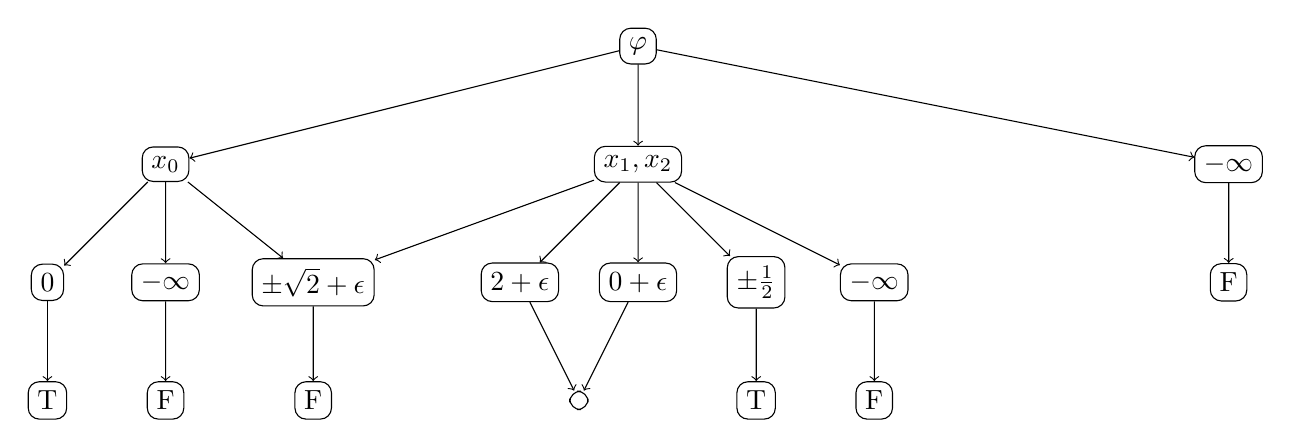
\begin{tikzpicture}[scale=1.5, 
				    state/.style={draw, rounded corners, fill=none,
				    			  text centered, text=black}]
	\node[state] (u1) at (5, 4) {$\varphi$};
	\node[state] (u2) at (1, 3) {$x_{0}$};
	\node[state] (u3) at (5, 3) {$x_{1},x_{2}$};
	\node[state] (u4) at (10, 3) {$-\infty$};
	\node[state] (u5) at (0, 2) {$0$};
	\node[state] (u6) at (1, 2) {$-\infty$};
	\node[state] (u7) at (2.25, 2) {$\pm\sqrt{2}+\epsilon$};
	\node[state] (u8) at (4, 2) {$2+\epsilon$};
	\node[state] (u9) at (5, 2) {$0+\epsilon$};
	\node[state] (u10) at (6, 2) {$\pm\frac{1}{2}$};
	\node[state] (u11) at (7, 2) {$-\infty$};
	\node[state] (u12) at (10, 2) {F};
	\node[state] (u13) at (0, 1) {T};
	\node[state] (u14) at (1, 1) {F};
	\node[state] (u15) at (2.25, 1) {F};
	\node[state] (u16) at (4.5, 1) {\lightning};
	\node[state] (u18) at (6, 1) {T};
	\node[state] (u19) at (7, 1) {F};

	
	\path[->] 	(u1)  edge   (u2);
	\path[->] 	(u1)  edge   (u3);
	\path[->] 	(u1)  edge   (u4);
	\path[->] 	(u2)  edge   (u5);
	\path[->] 	(u2)  edge   (u6);
	\path[->] 	(u2)  edge   (u7);
	\path[->] 	(u3)  edge   (u7);
	\path[->] 	(u3)  edge   (u8);
	\path[->] 	(u3)  edge   (u9);
	\path[->] 	(u3)  edge   (u10);
	\path[->] 	(u3)  edge   (u11);
	\path[->] 	(u4)  edge   (u12);
	\path[->] 	(u5)  edge   (u13);
	\path[->] 	(u6)  edge   (u14);
	\path[->] 	(u7)  edge   (u15);
	\path[->] 	(u8)  edge   (u16);
	\path[->] 	(u9)  edge   (u16);
	\path[->] 	(u10)  edge   (u18);
	\path[->] 	(u11)  edge   (u19);
\end{tikzpicture}
